\documentclass[tikz,border=5mm]{standalone}
\usetikzlibrary{patterns}
\begin{document}
	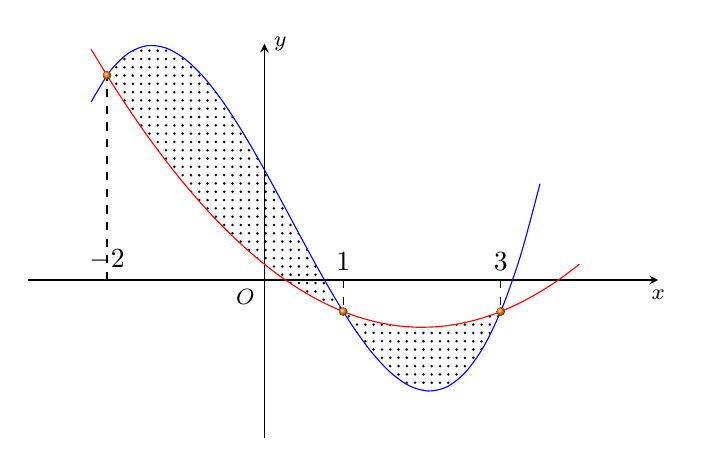
\begin{tikzpicture}[>=stealth]
		\def\f(#1){.2*((#1)^2-4*(\x)+1)}
		\def\g(#1){.2*( (#1)^3 -(#1)^2-9*(#1)+7)}
		\draw[->] (-3,0)--(0,0) node[below left]{\footnotesize $O$} --(5,0) node[below]{\footnotesize $x$};
		\draw[->] (0,-2)--(0,3) node[right]{\footnotesize $y$};
		\fill[pattern = dots,opacity=2] plot[domain=-2:3] (\x,{\f(\x)})--plot[domain=3:-2] (\x,{\g(\x)})--cycle;
		\draw[red,smooth] plot[domain=-2.2:4](\x,{\f(\x)});
		\draw[blue,smooth] plot[domain=-2.2:3.5] (\x,{\g(\x)});
		\foreach \x in {-2,1,3}{
			\draw[dashed] (\x,0)node[above]{$\x$}--(\x,{\f(\x)});
			\fill[ball color=orange] (\x,{\f(\x)}) circle (1.5pt);
		}
	\end{tikzpicture}
\end{document}